\chapter{Plano de Integração}

O plano de integração foi planejado, como mostra a Figura \ref{fig:planejamento_integracao}, onde todos os subsistemas se comunicam.

\begin{figure}[H]
    \centering
    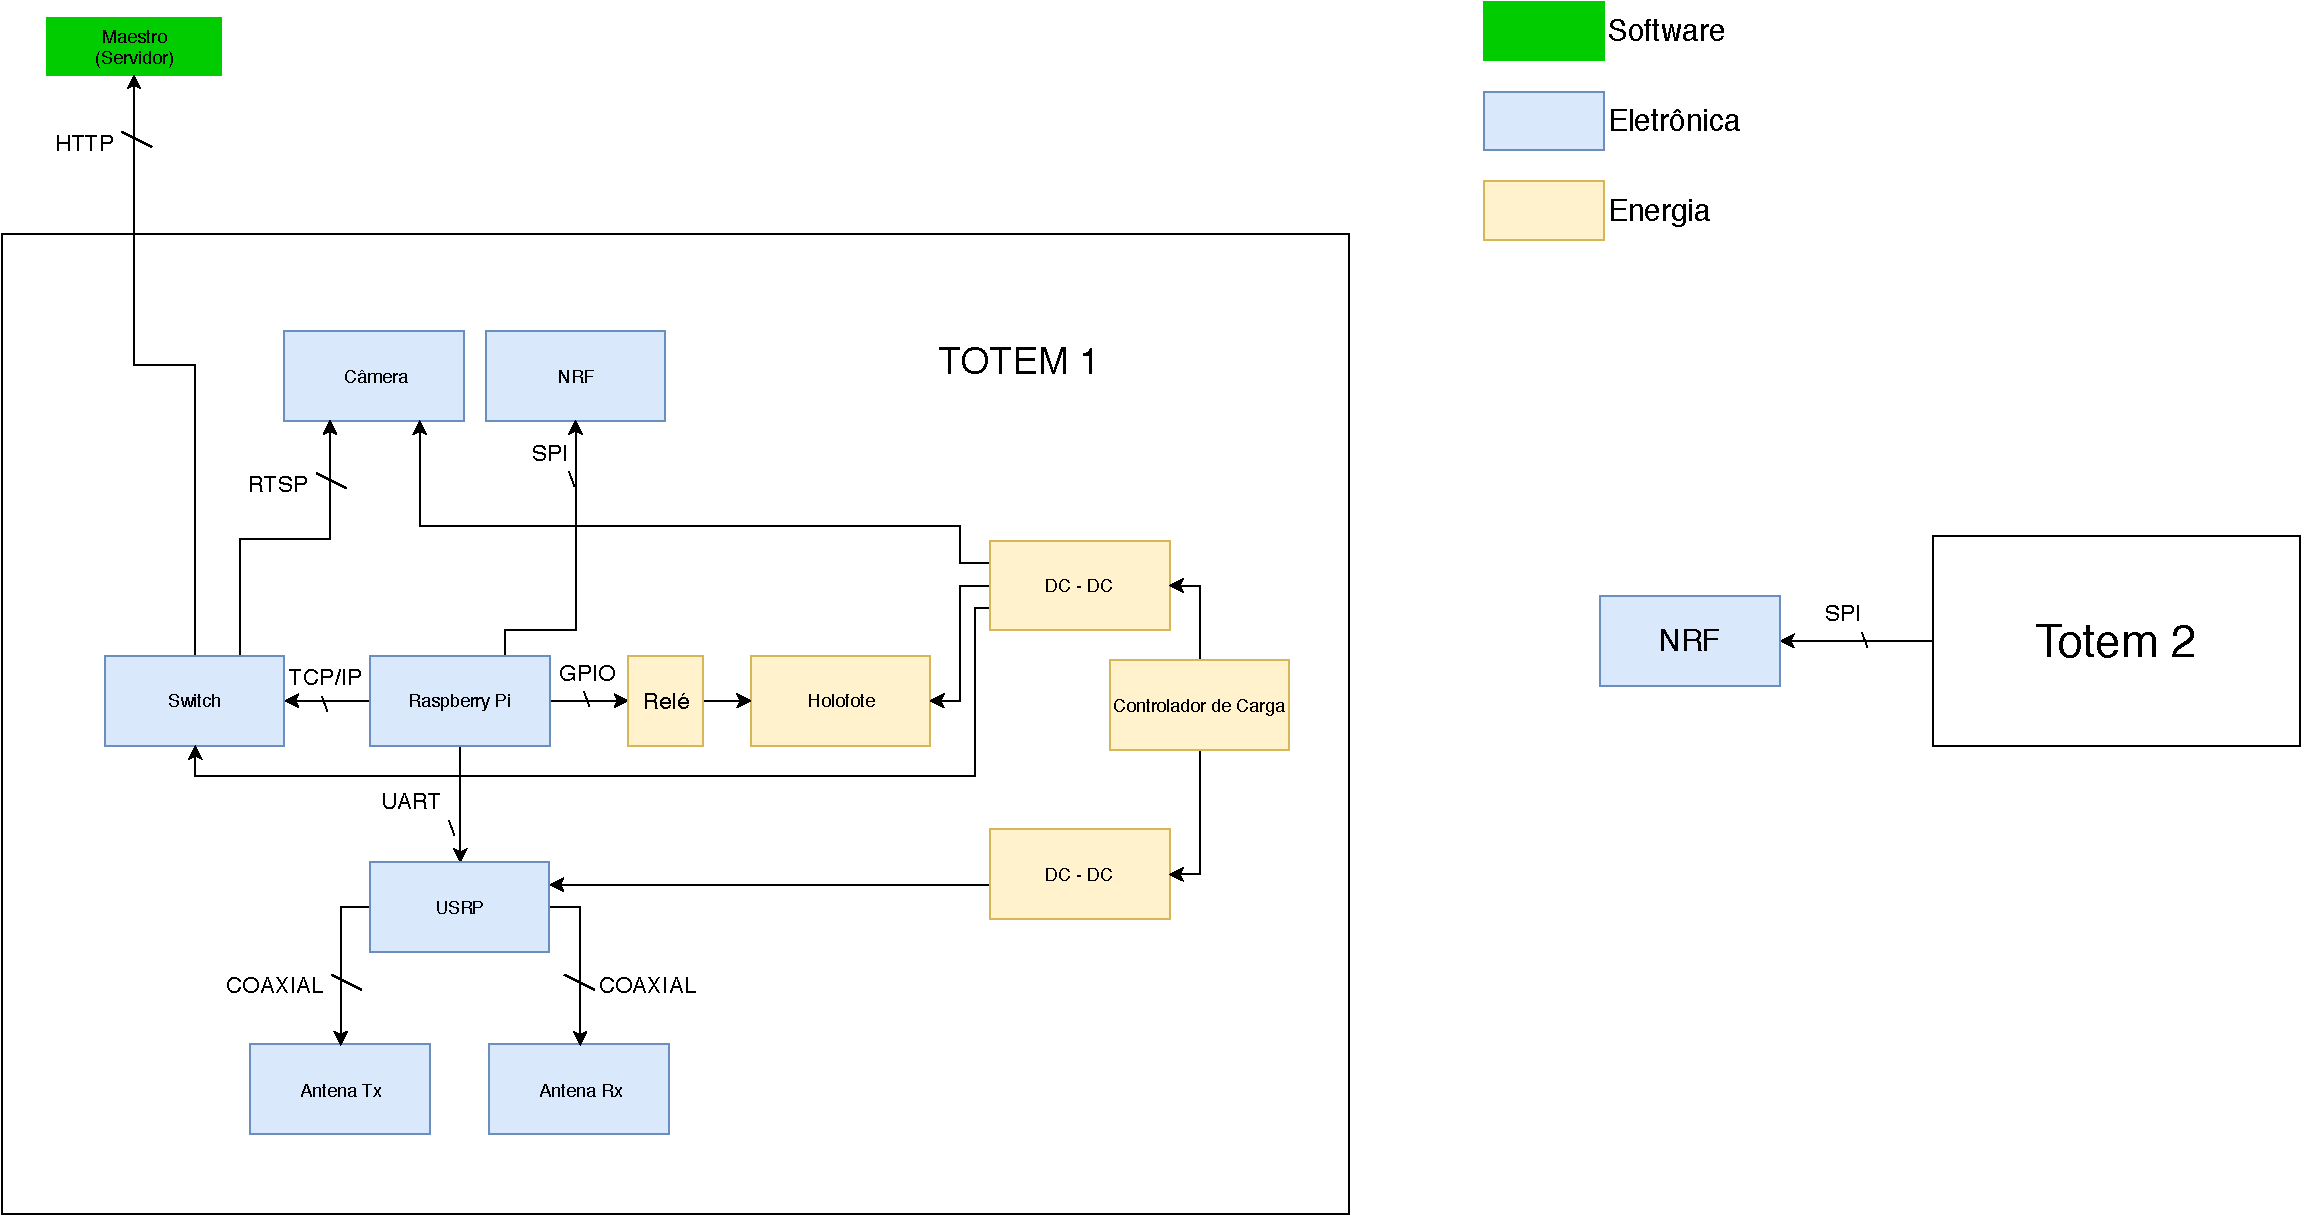
\includegraphics[scale=0.4]{geral}
    \caption{Diagrama de integração dos subsistemas.}
    \label{fig:planejamento_integracao}
\end{figure}

A primeira integração será feita entre o subsistema de energia e eletrônica onde, a alimentação do sistema do radar será distribuída através do subsistema painel fotovoltaico-baterias e subsistema composto por todos os componentes eletrônica presentes no radar. Esta integração será feita por meio do diagrama de fiação, onde os painéis fotovoltaicos são interligados as baterias e ao controlador de carga, sendo o controlador de carga o responsável pelo o controle de distribuição de energia aos componentes.

A segunda integração será feita entre o subsistema de software e eletrônica, onde os dados adquiridos pelo o subsistema de eletrônica serão enviados via comunicação TCP/IP para o Maestro, orquestrador dos subsistemas de software. Os dados relacionados que serão enviado são, o ID (identificador) do radar, a velocidade regulamentada, a velocidade medida, a velocidade considerada, a penalidade (grau), a data e hora das informações, as imagens das placas, as informações da câmera, operacionalidade da \emph{Raspberry} e USRP.

A terceira integração será feita entre o subsistema de estrutura e eletrônica, onde será instalado os componentes eletrônicos, a distribuição da fiação, antenas e câmera e os suportes das antenas e câmera, sendo estes a localização e distribuição correta no subsistema de estrutura.

A quarta integração será feita entre o subsistema de estrutura e energia, onde será instalado os painéis fotovoltaicos, as baterias, o dispositivo contra surtos, o controlador de carga e sua fiação, sendo estes a localização e distribuição correta no subsistema de estrutura.

A quinta integração é a emulação e comunicação entre a \emph{Raspberry} com o segundo radar, que está sendo realizada pelo o subsistema de eletrônica.

A última integração é constituída entre todos os subsistemas juntos, e será realizada logo após todas as anteriores terem serem concluídas, resultando no produto final da matéria.